\chapter{Эксперимент 2}

\section*{Исследование ВАХ полупроводниковых диодов с использованием мультиметров}

\begin{enumerate}
	\item Сначала я собрал схему, которая включала два мультиметра, резистор на 1 Ом, источник напряжения на 2 В, заземление и диод KD209A для измерения прямого тока.
	\begin{figure}[H]
		\centering
		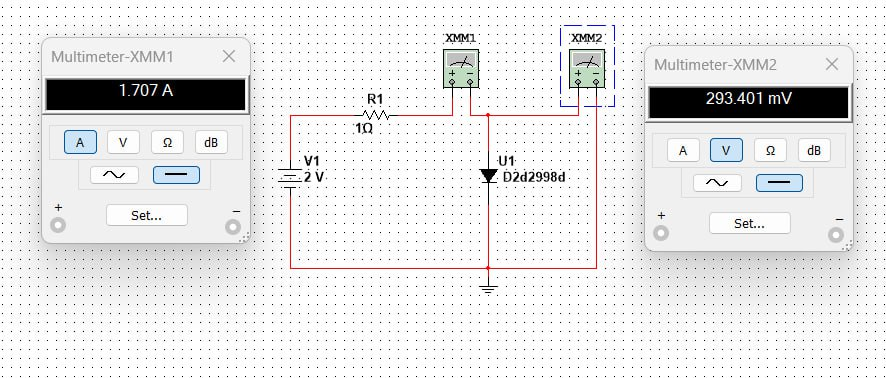
\includegraphics[width=0.6\textwidth]{img/11.jpg}
	\end{figure}
	\item Затем провел измерения и построил вольт-амперную характеристику для прямого тока.
	\begin{figure}[H]
		\centering
		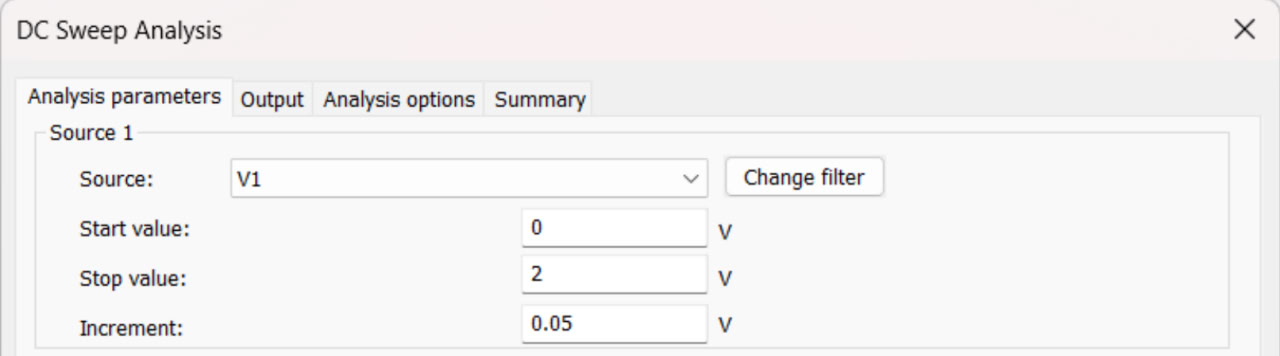
\includegraphics[width=0.6\textwidth]{img/dop_01.jpg}
	\end{figure}
	\begin{figure}[H]
		\centering
		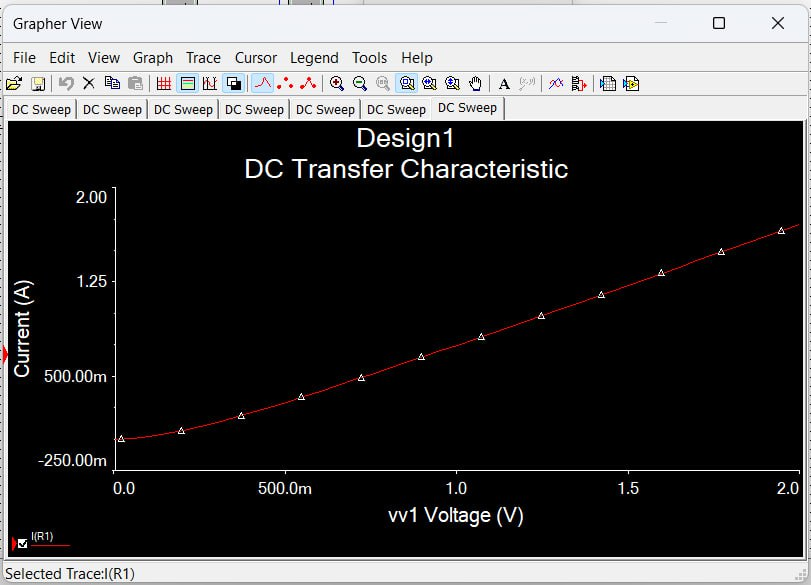
\includegraphics[width=0.6\textwidth]{img/12.jpg}
	\end{figure}
	\item После этого пересобрал схему для измерения обратного тока, развернув диод.
	\begin{figure}[H]
		\centering
		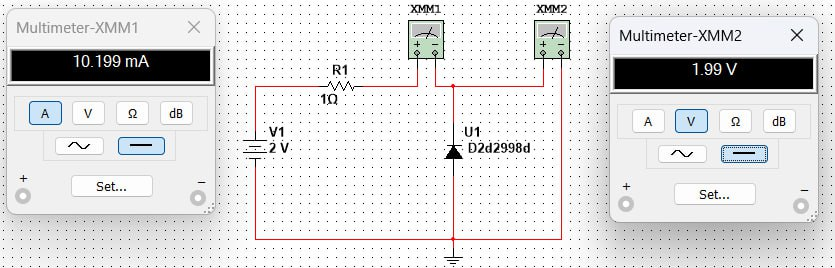
\includegraphics[width=0.6\textwidth]{img/13.jpg}
	\end{figure}
	\item Затем выполнил измерения и построил вольт-амперную характеристику для обратного тока.
	\begin{figure}[H]
		\centering
		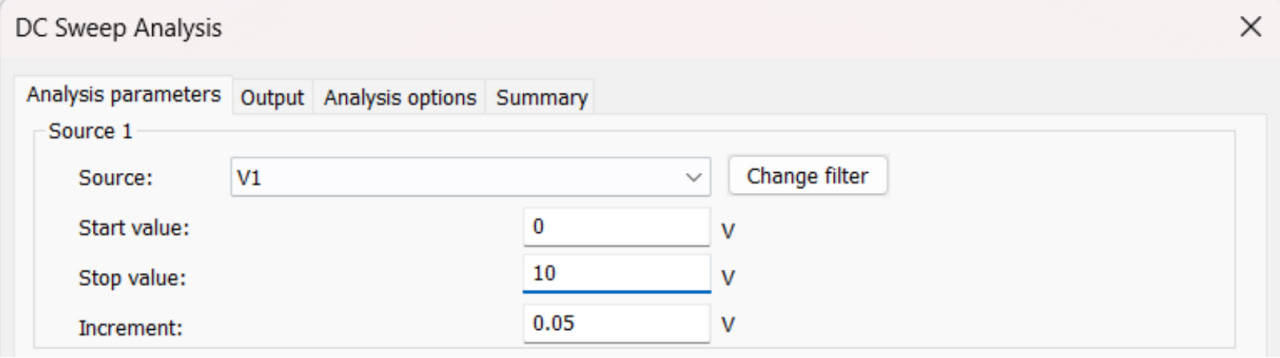
\includegraphics[width=0.6\textwidth]{img/dop_02.jpg}
	\end{figure}
	\begin{figure}[H]
		\centering
		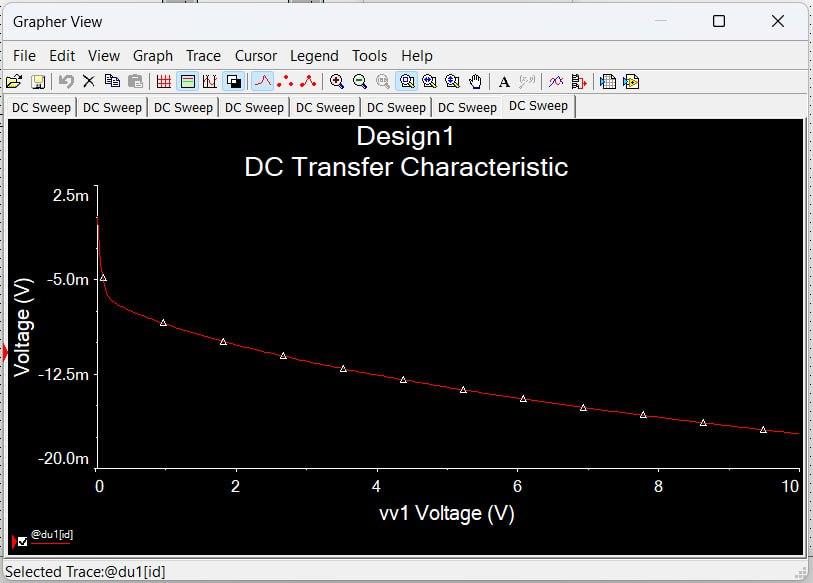
\includegraphics[width=0.6\textwidth]{img/14.jpg}
	\end{figure}
\end{enumerate}
